\documentclass[a4paper,12pt]{report}

\usepackage[frenchb]{babel}
\usepackage[utf8]{inputenc}
\usepackage[top=3cm, bottom=3cm, left=2.8cm, right=2.8cm]{geometry}
\usepackage{algorithm,algorithmic}
\usepackage{graphicx}


%Les 4 lignes suivantes servent à modifier les puces : plus seulement des tirets.
\renewcommand\labelitemi{\textbullet}
\renewcommand\labelitemii{\normalfont\bfseries\textendash}
\renewcommand\labelitemiii{\textasteriskcentered}
\renewcommand\labelitemiv{\textperiodcentered}

\title{Navigation dans un environnement 3D \vspace{0.5cm}}
\author{Marc BEYSECKER, Tom GIMENEZ, Valentin HIRSON, Léo RIZZON\\  \\Professeur encadrant : Mr Frédéric Koriche \\ \\Université Montpellier II \\  \\Master 1 Informatique}


\date{}
\begin{document}


\maketitle

\tableofcontents

\newpage

\chapter*{Remerciements}

Nous tenons à remercier M. Frédéric Koriche, notre encadrant de projet, pour avoir été disponible et attentif quand nous en avions besoin. Il nous a fait partager son savoir et a mis à notre disposition tous les outils dont nous avons eu besoin.

Son expérience et sa pédagogie nous ont permis de trouver nos repères dans ce vaste domaine qui nous était inconnu.

\chapter{Introduction}


\section*{Contexte}

Dans les jeux vidéos, les personnages non joués par des humains doivent pouvoir se déplacer de manière autonome et cohérente. Un environnement 3D est constitué d'un graphe énorme avec des milliers de sommets. Même en ne prenant que le sol, le graphe est encore très gros et, surtout, n'est pas seulement constitué des points naviguables. C'est à dire que le personnage ne doit pas pouvoir se déplacer dessus.

Comme nous l'avons étudié, la recherche de chemins dans un graphe est un problème classique mais qui peut s'avérer très lourd sur de gros graphes. En prenant en compte que les jeux mettent en scène un grand nombre d'agents il s'agit de minimiser les temps de calculs. 

Il s'agit donc d'une part de ne sélectionner que les points navigables et de simplifier le graphe obtenu pour limiter les espaces de calculs. De ces opérations nait le graphe des way-points. Il s'agit donc du graphe sur lequel vont se déplacer les agents.

Dans la plupart des jeux actuels les environnements sont créés ``à la main'' par les créateurs du jeu et les game designers placent eux même les points du graphe des way-points. Cela représente un gros travail et c'est même impossible dans le cas d'environnements aléatoirement générés.

Dans le cadre de notre unité d'enseignement intitulée Algorithmes de l'Intelligence Artificielle, nous avons réalisé un projet qui consiste en l'implémentation d'un algorithme de génération automatique du graphe des way-points.


\section*{Objectifs}

La base de notre travail est une scène 3D créée à l'aide d'un logiciel d'édition d'objets 3D, par exemple Blender. Il s'agit alors de charger cette scène pour y appliquer nos traitements. Tout d'abord, il faut générer le graphe à partir de tous les points composants les différentes formes pour représenter les arêtes. Ensuite il faut épurer ce graphe pour ne garder que les sommets et les arêtes ``empruntables``. Enfin on va chercher à appliquer un algorithme de simplification pour ne garder que les points réellement utiles. C'est une procédure appelée merging.

Le résultat serait donc un graphe des way-points, simplifié, automatiquement généré.

\chapter{Recherches préliminaires}

\section{Une scène en 3D avec Blender}

Blender est un logiciel d'édition d'objets 3D libre sous licence GPL. Bien que nous ayons eu la possibilité d'utiliser des logiciels payant très évolués, nous avons fait le choix, approuvé par notre professeur encadrant, d'utiliser Blender. Blender est multi-platerformes et c'est cet aspect qui nous a décidé car nous travaillons tous sous Linux. Bien que gratuit, il offre largement toutes les fonctionnalités dont avions besoin.

\subsection{Le maillage}

Pour simuler le travail sur un terrain assimilable à un environnement 3D de jeux vidéo, il nous fallait un graphe avec beaucoup de points. L'objectif était de passer 

Créer une scène simple sous Blender a été plutôt facile. Pourtant nous avons eu plus de mal à obtenir un maillage. Nous avons alors exploré plusieurs possibilités.

\paragraph{Une map Half-Life}

Au départ, nous avions dans l'idée de partir d'une map Half-Life. Dans un premier temps nous générions la map avec un générateur de terrain : Gensurf. Ensuite nous l'importions et l'éditions avec l'éditeur de map officiel WorldCraft. Nous arrivions donc à générer une scène rapidement et plus facilement qu'avec Blender. 
Malheureusement l'éditeur de map WorldCraft ne permet pas d'exporter directement en .obj , après quelques recherches, nous avons contourner le problème en utilisant Object Viewer qui permet de transformer un .map en .obj.

Au final, nous n'avons pas retenue cette solution car le .obj obtenu n'était pas aussi "propre" que celui obtenu par Blender. De plus la scène avait une épaisseur, ce qui ne nous plaisait pas.

\paragraph{Division directement dans notre programme}

Une autre solution que nous avons expérimentée, était de créer le maillage de notre scène par notre programme. Nous partions donc juste d'une forme carrée ou rectangulaire représentant le sol, puis nous la divisions en 4, ainsi de suite jusqu'à obtenir un maillage suffisant.
L'avantage de cette solution est que le designer n'est pas obligé de créer le maillage, il peut donc dessiner la scène qu'il veut sans trop de contraintes. Mais cette méthode présente des inconvénients : elle limite le contrôle sur la scène, elle rendait notre programme plus lourd et il fallait quand même passer par Blender pour créer la scène. Nous n'avons donc pas retenue cette solution.

\paragraph{La solution avec Blender}

Pour fabriquer notre sol nous avons longtemps cherché un modèle pré-conçu mais cela s'avéra infructueux.
Nous avons alors découvert qu'il était possible de diviser une forme de base. Nous avons décider de prendre un simple carré, de l'agrandir à la taille souhaitée et de le diviser en autant de petites cases que nécessaires. Cela nous a donc donné notre maillage sur lequel poser nos formes.
Nous avons posé des pavés sur notre sol car se sont les formes que prennent les bounding box. Une bounding box est la forme simplifiée que prend un modèle 3D; cela permet de simplifier les calculs d'intersection entre la forme et son environnement.

\subsection{Les différents formats de fichier}

Une fois la scène créée sous Blender le logiciel nous proposait différents formats d'exportation. Il y en a un grand nombre et nous en avons étudié principalement deux.

\paragraph{COLLADA}

Collaborative Design Activity (abrégé en COLLADA, signifiant activité de conception collaborative) a pour but d'établir un format de fichier d'échange pour les applications 3D interactives.

COLLADA définit un standard de schéma XML ouvert pour échanger les acquisitions numériques entre différents types d'applications logicielles graphiques qui pourraient autrement conserver leur acquisition dans des formats incompatibles. Les documents COLLADA, qui décrivent des acquisitions numériques, sont des fichiers XML, habituellement identifiés par leur extension .dae («digital asset exchange», traduit par «échange numérique d'acquisition»).
C'est un format supportant la vaste majorité des fonctionnalités modernes
requises par les développeurs de jeux vidéo. 

Il fallait donc faire un choix, COLLADA étant plus conséquent que .obj, et le sujet de notre TER n'étant pas porté sur le format de notre scène, 
nous avons donc choisi de faire simple et de choisir .obj. De plus le format XML nous obligeait à utiliser des librairies dédiées, complexes et non standardisées, qui nous aurait pris beaucoup plus de temps pour écrire le parser.

\paragraph{Wavefront}

OBJ est un format de fichier contenant la description d'une géométrie 3D. Il a été défini par la société Wavefront Technologies. Ce format de fichier est ouvert et a été adopté par d'autres logiciels 3D (tels que Maya, 3D Studio Max, Lightwave et bien sur Blender) pour des traitements d'import / export de données.

Dans un fichier Wavefront (extension .obj), les formes sont stockées les unes après les autres. Les différentes entités sont écrites par bloc.
Donc, pour chaque forme les informations qui la concerne sont stockées ligne par ligne. Nous savons à quoi chaque information correspond grâce à la lettre clef qui débute la ligne ( par exemple: ''v'' pour un vertex ).
Les seules informations qui nous intéressent sont les vertex et les faces. 
Une ligne pour un vertex fournit la position de ce vertex (x, y, z) décrite comme suit ''v x y z'' par exemple ''v 2.0 2.0 3.0'' pour un vertex de coordonnées (2.0, 2.0, 3.0)
Une ligne pour une face fournit le numéro des vertex qui la composent écrit comme suit ``f num$_{1}$ ... num$_{n}$`` par exemple ``f 4 6 7 8 11 13`` pour une face constituée des vertices numéros 4, 6, 7, 8 et 11. Le numéro d'un vertex n'est pas explicitement donné mais il se déduit par son ordre d'apparition dans le fichier Wavefront. C'est un identifiant unique.

Voici un exemple de code dans un fichier .obj.

Ici il s'agit d'un simple carré. Une forme commence par la liste des points qui la constitue puis la liste de ses faces.

\begin{verbatim}
v 0 0 0 //premier point de la nouvelle forme
v 0 0 1
v 1 0 1
v 1 0 0
f 1 2 3 4 //première face constituée des points 1 2 3 4
v ... //un v après un f on est donc sur une nouvelle forme
\end{verbatim}

Nous avons donc choisi ce format de fichier pour stocker notre scène 3D car il nous a été très facile de développer le parser adéquat. Les informations fournies sont justes celles dont nous avons besoin. On peut noter toutefois qu'il est possible d'exporter également des données sur les textures et les normales mais nous n'utilisons pas ces fonctionnalités.

\section{Récupérer notre scène en 3D}
 
Une fois notre scène créée sous Blender s'est posé le problème de l'exploiter. Nous avons alors cherché du côté des librairies existantes, en C/C++ surtout. En effet, Blender nous proposait divers formats de fichier de sortie. Nous devions faire en sorte que les informations soient récupérables et exploitables pour nos algorithmes. L'idée générale était d'utiliser un parser qui va lire les données du fichier pour les transformer en données compréhensibles par notre programme.

Voici les solutions que nous avons envisagées.
 
\subsection{OpenSceneGraph}

OpenSceneGraph est une extension d'OpenGL qui facilite le traitement d'une scène 3D. Elle permet de charger simplement des scènes dans des formats divers et de parcourir et d'agir sur les informations ainsi recuperées.
Une fois chargée, cette scène est transformée en un graphe très complexe contenant une énorme quantité d'informations. Ce graphe met en relation les formes entre elles et entre leurs informations respectives (textures, transformations, etc).
Cette solution n'a pas été retenue car nous n'avions pas le contrôle total de l'exécution d'OpenSceneGraph et la masse d'informations générée était plus une gène qu'un atout. Enfin la facilité de chargement de la scène réduisait l'intérêt de notre projet.

\subsection{OpenGL avec nos propres structures de données}

Une fois l'expérience OpenSceneGraph terminée et mise de côté, nous avons dû de nouveau chercher une solution. Après de longues recherches, nous avons trouvé quelques possibilités comme OGRE (Object-Oriented Graphics Rendering Engine), nous avons finalement décidé de créer nous même ce dont nous avions besoin. C'est la solution finale.

L'utilisation d'OpenGL (Open Graphics Library), conseillée par notre professeur encadrant, était un choix établi. C'est une spécification qui définit une API multi-plateforme pour la conception d'applications générant des images 3D (mais également 2D). Bien connue pour son ouverture, sa souplesse d'utilisation, sa stabilité et sa disponibilité sur toutes les plates-formes, OpenGL est de plus le sujet de nombreux tutoriaux. Elle est utilisée dans certains jeux-vidéo.

OpenGL nous a permis d'afficher notre graphe en 3D avec les points, les arêtes, les formes. Grâce à la gestion des vertices nous avons pu avoir un rendu des formes, utiliser la coloration des objets et créer un élément mobile représentant un agent. La caméra, bien gérée par cette librairie, a permis un gain de précision et de liberté d'observation dans notre affichage.

Enfin OpenGL est au programme de l'année prochaine : il est toujours intéressant de prendre un peu d'avance. 

Au niveau du langage de programmation, coder en C++, pour la performance du programme, pour l'aspect objet intéressant dans notre contexte, pour l'utilisation d'OpenGL, était presque évident.

Finalement nous avons donc implémenté notre propre parser pour remplir nos propres structures de données. En fait, nous avons recodé une partie des fonctionnalités des librairies que nous avions étudiées pour n'en garder que ce dont nous avons besoin et pour avoir des structures que nous maitrisions pleinement. Au final, cela nous a fait gagné du temps.

\section{Test de validité des points : Bounding Box}

Pour tester si un point est valide nous avons dû réfléchir à quelle méthode utiliser. Notre professeur encadrant nous avait parlé de Bounding Box.

Les Bounding Box sont des objets invisibles générés à partir d'autres objets. Chaque Bounding Box est un cube (ou un prisme à base rectangulaire) et contient une forme. Elle représente l'objet de manière simplifiée. Cela permet de réduire la complexité de différents calculs, tels que les collisions entre deux formes lors de la recherche de chemins.

Dans notre cas elles sont utiles pour détecter les sommets invalides du graphe des way-points. Nous avons commencé par faire abstraction de la hauteur, car lorsque nous parcourons le graphe nous ne savons pas quelles sont les caractéristiques des formes qui vont se déplacer.Nous ne connaissons ni la nature du sol (eau, terre, lave...) ni les attributs de la forme ou de l'agent (taille, largeur, capacité à voler ou nager...). Comme il nous manque des éléments sur la hauteur pour affiner les opérations sur le graphe en fonction de qui parcourt ce graphe, Nous avons décidé que, peu importe la hauteur (axe Y) d'un objet, il est impossible circuler sur l'espace où est projeté une forme sur le graphe. 

\begin{figure}[!ht]
\centering
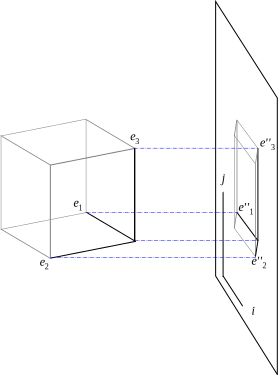
\includegraphics[scale=0.6]{Images/Projection_orthogonale_illustration.jpg}
\caption{Exemple de projection orthogonale d'un carré sur un plan 2D}
\end{figure}
\vspace{0.5cm}

\newpage
De là nous avons besoin de seulement quatre points pour représenter notre Bounding Box. Nous utilisons des vertex, comme cela, si nous voulons étendre notre modèle à des Bounding Box en trois dimensions il suffit de rajouter quatre autres vertex.

\chapter{Implémentation finale}

Nous présenterons ici les éléments que nous avons effectivement implémentés. Le travail en équipe a nécéssité une bonne organisation et nous avons créé un SVN et un Google Group.

\section{Principe général}

Voici le principe général de notre programme. Ci-après les différentes étapes successives en considérant que l'on part d'une scène 3D en format Wavefront.

\begin{itemize}
 \item Parser le fichier .obj de la scène 3D
 \item Isoler le sol des autres formes
 \item Générer le graphe correspondant au sol
 \item Détecter les sommets invalides et les retirer du graphe
 \item Simplifier le graphe (merging)
\end{itemize}

\section{Nos structures de données}

Nous présenterons ici nos structures de données, utilisées dans notre projet. Comme dit précédemment, nous avons exploité le potentiel objet du C++ et la liste suivante énumère des classes.

\begin{itemize}
 \item Forme:

Une \textit{forme} est une figure géométrique qui contient une liste de vertex et une liste de faces. À partir d'une forme, nous pouvons générer un graphe qui lui correspond.
 
 \item Vertex:

Un \textit{vertex} est un point de notre scène. Il possède 3 coordonnées x, y et z. Il contient également une liste de pointeurs sur les vertices qui sont ses voisins.

 \item Faces:

Les \textit{faces} possèdent une liste contenant les numéros des vertex qui les composent. C'est grâce aux faces que nous pouvons déduire les voisins des sommets du graphe. Elles servent aussi à effectuer un affichage cohérent des formes.

 \item Bounding Box:

Les \textit{Bounding Box} possèdent 4 vertices qui correspondent aux points de la projection en 2D de la Bounding Box sur le sol. La classe possède un constructeur qui prend une forme en paramètre, on y calcule la Bounding Box d'une forme quelconque.

\end{itemize}


\subsection{La scène}

Reprécisons bien comment sont stockées les données.

Notre scène, c'est à dire l'ensemble de tous les vertices et de toutes les formes, est stockée dans une liste de formes. On a donc, comme expliqué plus haut, une scène complète séparée en différentes formes : par exemple une forme qui correspond à tout le sol, une à un cube, etc.

C'est pourquoi nous avons une méthode qui permet d'identifier quelle forme est le sol. Dans notre cas, nous avons pu faire très simple : la forme correspondant au sol est celle qui possède le plus de points. On peut noter que notre sol peut contenir des points avec une hauteur différente de 0 (relief).

\subsection{Le graphe généré}

Pour stocker notre graphe dont la création est expliquée plus loin, nous avons fait le choix de rajouter à notre classe Vertex une liste d'adjacence contenant des pointeurs vers les voisins de ce sommet. C'est donc une méthode d'implémentation classique où chaque sommet connait ses voisins. Encore une fois, comme le point principal du projet n'est pas là, nous avons choisi de faire au plus simple. 

Grâce à cette liste de voisins (ou d'adjacences), les parcours dans le graphe sont possibles (cette liste représente les arêtes du graphe). Nous avons choisi les listes de voisins car chaque sommet possède au plus 4 voisins si le maillage est fait de carrés ou 3 voisins s'il est fait de triangles. Ce qui permet un coût de stockage très faible et un temps de calcul bien maitrisé. 

Prenons l'exemple de la suppression d'un voisin :

Il suffit de l'isoler pour qu'il ne soit plus parcouru ; soit le supprimer de la liste de voisins de tous ses voisins. Au pire des cas: 4 x 4 tests.
 
Cette liste d'adjacence est donc remplie à l'appel de la méthode de génération du graphe.

\section{Un parser pour récupérer notre scène}

Nous récupérons donc un fichier au format Wavefront. Il s'agit de remplir nos structures de données, un vecteur de forme que nous appelerons ici \textit{listeDeFormes}.
Nous avons présenté précédemment la structure d'un fichier au format Wavefront. Ici nous présenterons le fonctionnement de notre parser.

\begin{algorithm}[h]
\caption{Parser de fichier .obj}
\label{parser}
\begin{algorithmic}[1]
\REQUIRE fichier .obj
\FOR{chaque forme (c'est à dire une apparition de ''v`` après une série de ''f'')}
  \IF{la ligne commence par un ``v''}
    \STATE enregister ``v x y z'' comme nouveau vertex de coordonnées (x,y,z) dans le vecteur de vertex de la forme courante
  \ELSE
    \IF{la ligne commence par un ``f''}
    \STATE enregistrer ``f $x_{1}$ ... $x_{n}$'' comme nouvelle face dans le vecteur de faces de la forme courante
    \ENDIF
  \ENDIF
\ENDFOR
\end{algorithmic}
\end{algorithm}

\section{Génération du graphe correspondant au sol}

Pour effectuer les traitements prévus nous avons donc décidé de travailler sur un graphe. Nous partons d'un ensemble de points et de faces dans des formes séparées. Nous sélectionnons la forme correspondant au sol avec notre méthode dédiée. Ensuite, sur cette forme nous appliquons une méthode qui va créer les liaisons entre sommets en fonction des faces de la forme. 

Pour chaque face on lie ses vertices de manière à ce que chaque sommet prenne comme voisins son prédecesseur et son successeur dans leur ordre d'apparition de la liste des points de la face.

Notre sol n'est composé que de carrés et chaque face possède une liste de 4 sommets A,B,C,D.

voisins(A) = {B,D} ;  voisins(B) = {A,C} ; voisins(C) = {B,D} ; voisins(D) = {A,C}

\section{Travaux effectués sur le graphe}

Notre scène est donc récupérée dans notre programme. Nous avons de plus généré le graphe du sol. Il nous faut maintenant y appliquer nos traitements.

\subsection{Création du graphe des way-points}

Dans un premier temps, à partir de tous les points du graphe, nous allons chercher à supprimer tous les point sur lesquels un agent ne doit pas pouvoir se déplacer. Nous obtiendrons ainsi le graphe des way-points, ensemble des points navigables.

\subsubsection{Parcours}

Voici notre méthode de parcours, en profondeur. 

\begin{algorithm}[h]
\caption{Parcours du graphe complet : parcourir(sommet)}
\label{parcours_graphe}
\mbox{Algorithme lancé à partir d'un sommet non isolé}
\begin{algorithmic}[1]
\IF{sommet courant non marqué}
  \STATE marquer le sommet courant
  \FOR{chaque voisin v}
    \STATE parcourir(v)
  \ENDFOR
\ENDIF
\end{algorithmic}
\end{algorithm}

\subsubsection{Heuristique}

Notre heuristique, qui va déterminer si un point est navigable ou pas va se baser sur les bounding box. Une bounding box est la plus petite boite englobant l'ensemble des points d'une forme. Générer une bounding box pouvant être un travail compliqué, nous avons choisi de dire que notre bounding box était constituée de quatres points (vertex). On calcule leurs coordonnées selon les valeurs minimales et maximales de tous les vertex d'une forme. On classe les quatres points afin de facilité les calculs à venir.

On considère comme valide :
\begin{itemize}
 \item un sommet s'il n'est pas contenu dans une bounding box. 
 \item une arête, entre deux sommets, si elle ne coupe pas une bounding box
\end{itemize}

Une arête, entre deux sommets, est valide si elle ne coupe pas une bounding box. Il nous a donc fallu implémenter deux méthodes renvoyant un prédicat pour savoir quels points et quelles arêtes supprimer. 
Quand un point est non valide, on l'isole dans le graphe. On peut afficher tous les points pour voir clairement les différences. Le parcours du graphe est quand à lui simplifié.

L'heuristique a été un pilier très important de ce projet et a été l'objet d'une réflexion assez poussée. Nous présenterons différentes méthode qui ont été envisagées.

\paragraph{Méthode 1 }
Cette solution, souvent utilisée en informatique, consiste à déterminer si un point (x,y) est à l'intérieur ou à l'extérieur d'un
polygone sur un plan 2D. 
Considérons un polygone, fait de n sommets (x$_{i}$,y$_{i}$) avec $i$ de $0$ à $n-1$. Le dernier sommet (x$_{n}$,y$_{n}$) est le même que le premier sommet, pour que le polygone soit fermé. 
Pour déterminer le statut d'un point (x$_{p}$,y$_{p}$), on trace une droite horizontale partant de (x$_{p}$,y$_{p}$). 
Si le nombre d'intersection de la droite avec chaque arête du poylygone est impair alors le point est à l'intérieur du polygone, sinon il n'est pas dedans.

\begin{figure}[h]
\centering
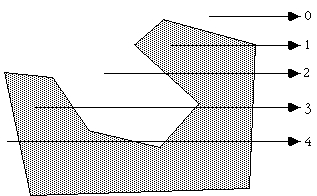
\includegraphics[scale=0.6]{Images/insidepoly1.jpg}
\includegraphics[scale=0.6]{Images/insidepoly3.jpg}
\caption{Différents cas de figures avec nombre d'intersection paire et impaire}
\label{nbintersect}
\end{figure}
\vspace{0.5cm}

Le seul problème apparait lorsqu'un sommet ou une arête du polygone est parallèle à la droite.

Les situations possibles sont illustrées en dessous :

\begin{figure}[h]
\centering
\includegraphics[scale=0.6]{Images/insidepoly2.jpg}
\caption{Illustration des épaisseurs de ligne}
\end{figure}
\vspace{0.5cm}

Les lignes épaisses ne sont pas considérées comme valides, les lignes fines si.
Il est bon de noter que cet algorithme marche avec des polygones troués, comme illustré sur le figure \ref{nbintersect}.

Cette méthode est idéale pour les polygones non convexes mais comme nous utilisons des carrés, elle aurait été un peu lourde.

\paragraph{Méthode 2 }
Une autre solution est de calculer la somme des angles fait entre le point test et chaque paires de points du polygone. Si la somme est égale à $2\pi$ alors le point est à l'intérieur, sinon le point est à l'extérieur. 
Cette méthode marche aussi avec les polygones troués.
De même cette méthode est assez gourmande en calcul et n'a pas été retenue.

\paragraph{Méthode 3 : retenue}
La dernière solution que nous avons testé ne marche qu'avec les polygones convexes. Si un polygone est convexe alors on peut considérer ces arêtes comme un "chemin" partant du premier sommet pour y revenir. 
Un point est à l'intérieur du polygone s'il est toujours du même côté que tous les arêtes constituant le ``chemin''.

\begin{figure}[h]
\centering
\includegraphics[scale=0.5]{Images/chemin2.jpg}
\caption{Un chemin dans un carré}
\end{figure}
\vspace{0.5cm}

Soit un segment entre P0(x$_{0}$,y$_{0}$), P1(x$_{1}$,y$_{1}$) et un autre point P(x,y) alors on a la relation suivante : (y - y$_{0}$).(x$_{1}$ - x$_{0}$) - (x - x$_{0}$).(y$_{1}$ - y$_{0}$).
Si le résultat est inférieur à 0 alors P est à droite du segment [P0,P1], s'il est égale à 0 alors il est sur la droite (P0,P1) et s'il est supérieur à 0 alors il est à droite du segment [P0,P1].

À noter que cet algorithme ne marche pas avec les polygones troués. 

Il nous suffit donc de faire 4 tests, on teste la position du point par rapport à chacune des arêtes constituant le polygone, si le point est toujours du même côté alors le point est à l'intérieur du polygone.

Nous avons choisi de retenir la solution 3 car c'est celle qui nous semblait fonctionner le mieux ainsi que la plus économe en ressources. Elle est parfaitement adaptée à notre projet.

\paragraph{Méthode de test d'intersection d'une arête avec une bounding box }

Pour tester si une arête coupe une bounding box nous avons décomposé le problème :
\begin{itemize}
 \item dans un premier temps il nous fallait une méthode pour savoir si un segment est coupé par un autre.
 \item ensuite il suffit de tester si notre arête coupe chaque segment de la bounding box, notre bounding box étant un carré on a donc 4 tests à faire.
\end{itemize}

L'intersection d'un segment avec un autre peut être un problème extrêment simple ou extrêment compliqué, dépendant de l'application. 
Mais si l'on veut seulement le point d'intersection alors la méthode suivante marche :

Soit A,B,C,D des vecteurs. Alors on a les propriétés suivantes :

$AB=A+r(B-A)$, $r \in [0,1]$


$CD=C+s(D-C)$, $s \in [0,1]$

\vspace*{3mm}
$r = \frac{(A_{y}-C_{y})(D_{x}-C_{x})-(A_{x}-C_{x})(D_{y}-C_{y})}{(B_{x}-A_{x})(D_{y}-C_{y})-(B_{y}-A_{y})(D_{x}-C_{x})}$
\vspace*{3mm}

$s = \frac{(A_{y}-C_{y})(B_{x}-A_{x})-(A_{x}-C_{x})(B_{y}-A_{y})}{(B_{x}-A_{x})(D_{y}-C_{y})-(B_{y}-A_{y})(D_{x}-C_{x})}$
\vspace*{3mm}

Après, le test est simple : 
\begin{itemize}
 \item Si $0\le r \le 1 \wedge 0 \le s \le 1 \rightarrow$ intersection
 \item Si $r<0 \vee r>1 \vee s<0 \vee s>1 \rightarrow$ pas d'intersection
\end{itemize}



Voici une illustration de l'application de l'heuristique dans un cas complexe avec des sommets invalides recouverts et des arêtes coupées par la forme sans que les sommets qu'elles relient soient invalides : 

\begin{figure}[h]
\centering
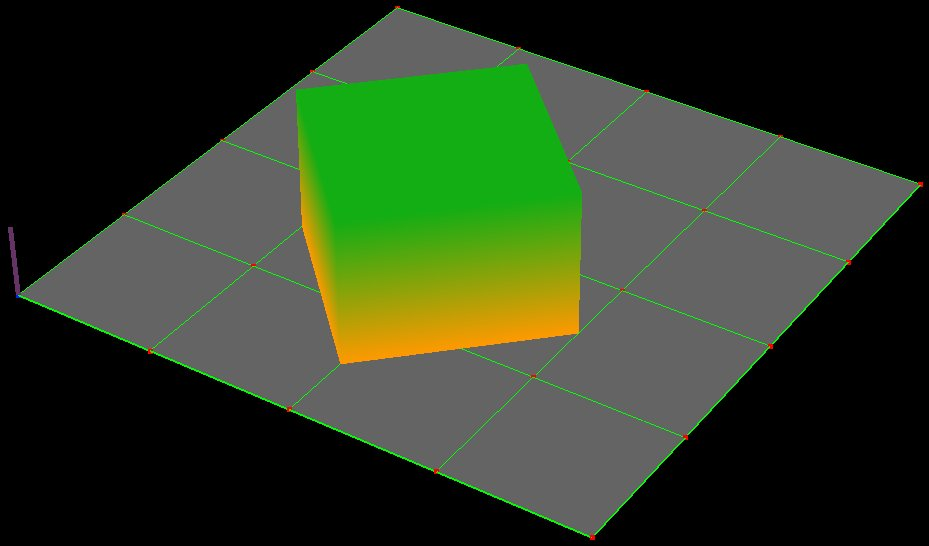
\includegraphics[scale=0.25]{Images/1-maillage.jpg}
\caption{Exemple de forme qui coupe des arêtes sans recouvrir les sommets qu'elles relient}
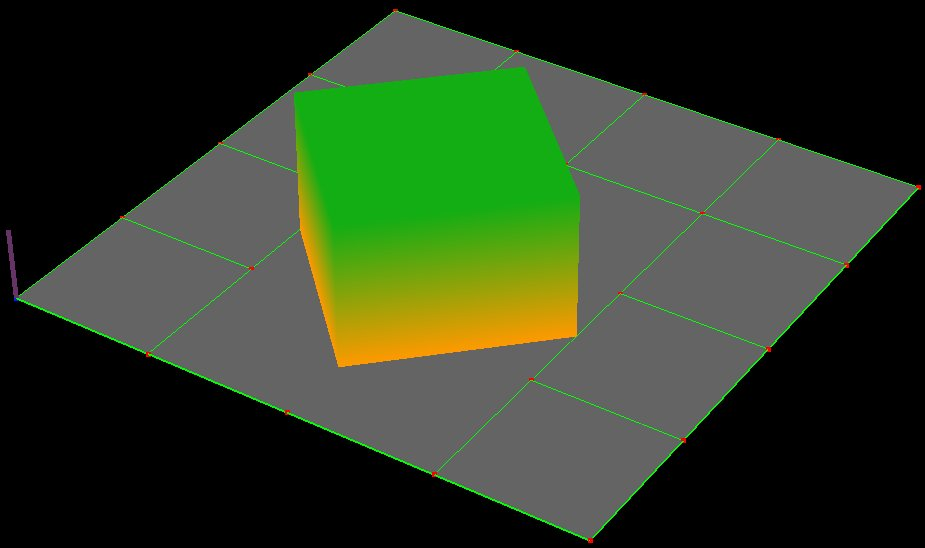
\includegraphics[scale=0.23]{Images/2-SuppressionSommet.jpg}
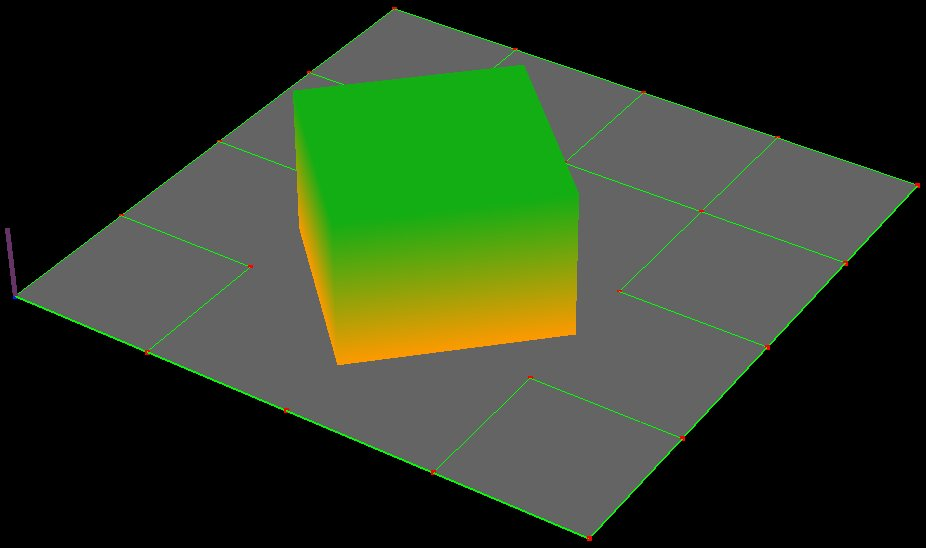
\includegraphics[scale=0.23]{Images/3-SuppressionAretes.jpg}
\caption{Dans un premier temps, suppression des sommets recouverts, ensuite suppression des arêtes invalides}
\end{figure}
\vspace{0.5cm}

Enfin, comme on ne travaille que sur une projection 2D, les reliefs ne posent pas problème et sont bien pris en compte. En contre-partie le sol qui passerait au dessus d'un obstacle sera innaccessible.

\newpage

\subsection{Simplification du graphe des way-points : merging}

Pour limiter les calculs de recherche de chemins les graphes des way-points sont généralement simplifiés par l'application d'une technique qu'on appelle merging. 

Nous n'avons pas eu le temps de développer un merging très évolué. Toutefois notre procédure de merging remplit son rôle en préservant la connexité du graphe. Il s'agit en fait d'isoler certains sommets dont l'entourage possède un grand nombre de voisins. 

\begin{algorithm}[!h]
\caption{Merging du graphe : merging(sommet)}
\label{merging_graphe}
\mbox{Algorithme lancé à partir d'un sommet non isolé}
\begin{algorithmic}[1]
\IF{sommet courant non marqué}
  \STATE dupliquer la liste des voisins
  \IF{sommet courant a 4 voisins}
    \IF{sommets voisins du sommet courant ont tous au moins 3 voisins}
      \STATE isolation du sommet courant
    \ENDIF
  \ENDIF
  \FOR{chaque voisin v sauvegardé}
    \STATE merging(v)
  \ENDFOR
\ENDIF
\end{algorithmic}
\end{algorithm}

\begin{figure}[!h]
\centering
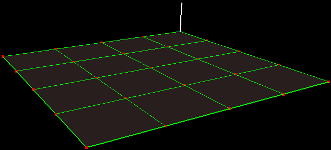
\includegraphics[scale=0.6]{Images/maillage.png}
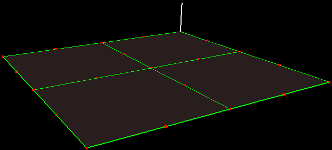
\includegraphics[scale=0.6]{Images/merging.png}
\caption{Notre graphe avant et après merging}
\end{figure}
\vspace{0.5cm}

\chapter{Résultats}

Ce chapitre est dédié à la présentation du résultat final à travers quelques exemples. Nous parlerons également de l'interface graphique mise au point pour afficher la scène et pour y appliquer nos différents traitements.

\section{Interface graphique}

Nous avons utilisé le gestionnaire de fenêtres de la libraire SDL pour contenir notre scène affichée. Cette librairie nous permet de récupérer les différents évenements, tels que les évenements clavier ou encore le redimensionnement de la fenêtre. Nous n'avons pas eu de problèmes particuliers liés à son installation ou à son utilisation.

Pour le rendu graphique 3D nous nous sommes donc servi d'OpenGL. Le résultat est l'affichage de notre scène avec la possibilité de l'explorer en déplaçant la caméra. Nous avons implémenté la gestion de différents événements clavier liés à nos traitements sur le graphe dont voici la liste :

\begin{itemize}
 \item[d] : détecter et enlever les points invalides avec suivi visuel (attention procédure longue)
 \item[a] : détecter et enlever les points invalides sans suivi visuel (procédure rapide)
 \item[z] : détecter et enlever les arêtes invalides
 \item[m] : merging, simplification du graphe
 \item[c] : afficher/masquer les formes
 \item[t] : afficher/masquer le graphe
 \item[touches directionnelles] : déplacement de la caméra
\end{itemize}


\section{Application de l'heuristique}

Donc, en appuyant sur la touche ``d'' ou ``a'' nous pouvons masquer, ou plutôt isoler les sommets invalides. Voici un exemple (pour plus de lisibilité nous avons choisi de ne pas afficher les formes qui couvraient les points en question : 

\begin{figure}[!h]
\centering
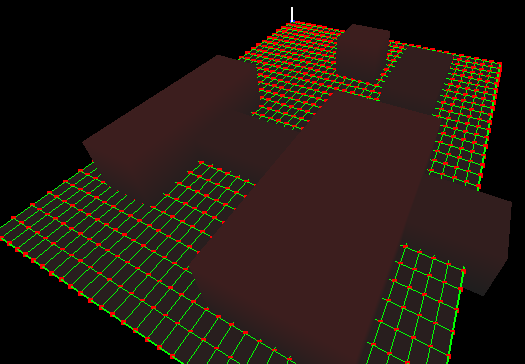
\includegraphics[scale=0.4]{Images/heuristique1.png}
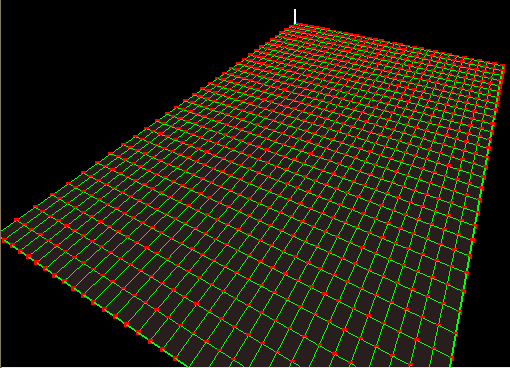
\includegraphics[scale=0.4]{Images/heuristique2.png}
\caption{Notre graphe avant application de l'heuristique, d'abord avec les formes affichées qui cachent les sommets en dessous puis avec les formes masquées}
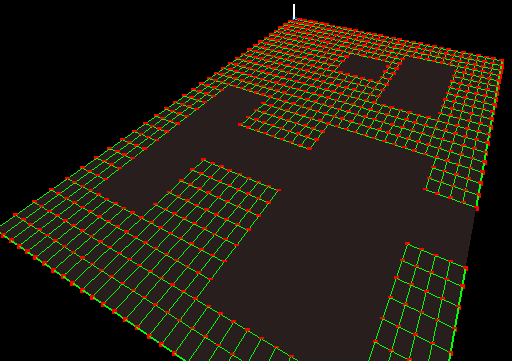
\includegraphics[scale=0.5]{Images/heuristique3.png}
\caption{Notre graphe après l'application de l'heuristique (formes non affichées)}
\end{figure}
\vspace{0.5cm}

\newpage

\section{Merging}
 
Avec la touche ``m'' du clavier on peut lancer la procédure de merging. Voici les résultats obtenu sur l'exemple précédent. Notons que l'application de l'heuristique doit avoir lieu avant. 

\begin{figure}[h]
\centering
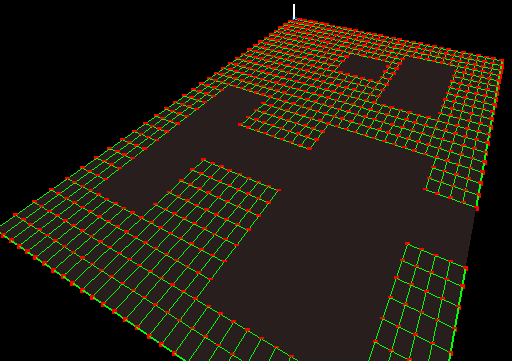
\includegraphics[scale=0.5]{Images/heuristique3.png}
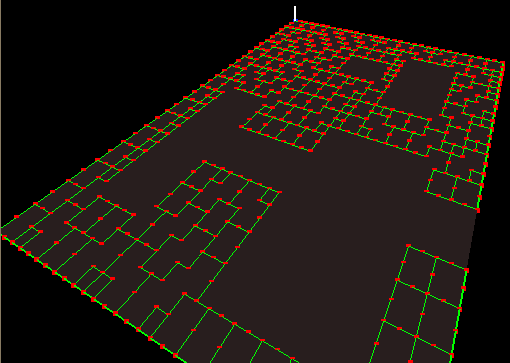
\includegraphics[scale=0.5]{Images/merging3.png}
\caption{Notre graphe après application de l'heuristique, avec les formes masquées, avant et après la procédure de merging}
\end{figure}
\vspace{0.5cm}

\newpage

\section{Déplacement d'un agent}

Pour mieux illustrer les déplacements possibles dans le graphe des way-points, nous avons implémenté la possibilité d'afficher et de déplacer un personnage en 3D.




Pour vérifier notre travail, pour une mise en condition ``réelle`` et pour un rendu encore plus sympathique, nous avons implémenté un agent qui va effectuer un parcours sur notre graphe. Il est modelisé par une ligne blanche.
Pour charger le modèle ( en .obj ), nous nous servons du parser que nous avons initialement créé pour charger la scène et nous obtenons toujours un vecteur de formes.
Toutes ces formes seront affichées en même temps que la scène et la position du personnage dépend du vertex qu'il a calculé avant de se déplacer.


Chaque sommet possède un poids, initialement nul, qui va augmenter de 1 à chaque passage de l'agent.

Pour bien voir le chemin parcouru, nous colorons les sommets parcourus en bleu avec une proportionnalité en fonction du poids. Plus le poids est élevé, plus le sommet s'éclairci.

Pour choisir le vertex vers lequel le personnage va se deplacer, celui-ci calcule le chemin de coût minimal entre sa position et un vertex de distance d. Son voisin lui renvoyant le coût minimal sera sa prochaine destination.

Notre algorithme de déplacement est le suivant : 

\begin{algorithm}[h]
\caption{Déplacement d'un agent : parcours(pas)}
\mbox{Algorithme lancé à partir du sommet courant de l'agent}
\begin{algorithmic}[1]
\IF{pas = 0}
  \STATE retourner monPoids
\ELSE
  \IF{monPoids = 0}
    \STATE retourner 0
  \ELSE
  \FOR{chaque voisin v $\ne$ monPère}  
      \STATE p = min\{p, v.parcours(pas - 1)\}
  \ENDFOR
  \STATE retourner monPoids + p
  \ENDIF
\ENDIF
\end{algorithmic}
\end{algorithm}

L'agent se déplacera donc sur le voisin débutant un chemin de poids minimal.

\begin{figure}[!ht]
\centering
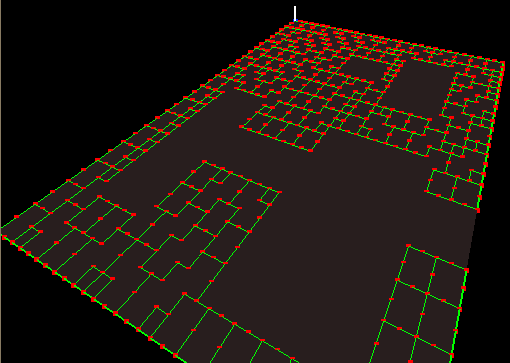
\includegraphics[scale=0.5]{Images/merging3.png}
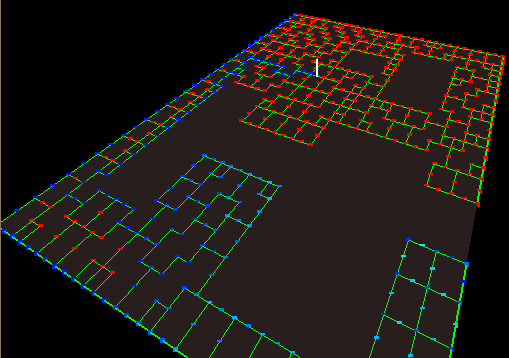
\includegraphics[scale=0.5]{Images/parcours1.png}
\caption{Notre graphe après application de l'heuristique, avec les formes masquées, après la procédure de merging, avant l'exploration et pendant l'exploration}
\end{figure}
\vspace{0.5cm}

\chapter{Conclusion}

\subsection*{Bilan technique}

Notre projet s'apparentait à un projet de recherche. Une grande partie du travail a donc consisté à explorer le domaine des environnements 3D. Nos objectifs principaux ont été atteints : nous créons une scène 3D avec un logiciel dédié, Blender ; nous la chargeons dans notre programme ; nous y appliquons les traitements prévus c'est à dire l'heuristique pour la suppression des sommets non navigables et le merging pour simplifier le graphe des way-points obtenu. Enfin nous avons un agent qui utilise un algorithme d'exploration plutôt évolué.

Nos structures de données, bien que parfaitement fonctionnelles, ne sont pas implémentées le plus ''proprement`` possible. Toutefois ce n'était pas l'objet principal du projet et nos avons fait le choix de nous concentrer sur d'autres points.

Notre parser est très simple et ne gère que les fichier .obj de base (sans texture, normales etc.). Encore une fois cela était parfait pour notre travail.

Les différents algorithmes par contre ont été le sujet de beaucoup d'attention. Les données pouvant être de très grande taille, en nombre de points et d'arêtes par exemple, nous avons été vigileant quand aux complexités.

La génération des Bounding Box étant un problème très complexe, nous avons fait le choix, en correlation avec notre projet, de le réduire au calcul de Bounding Box non minimales et effectives sur un plan 2D.

Le rendu à l'écran n'a pas été notre priorité mais il est clair, fonctionnel : largement suffisant pour y voir nos résultats.

Au final, notre agent peut se déplacer dans un environnement 3D, avec reliefs et obstacles, sans problème de collision. Son graphe des way-point est cohérent et auto-généré.

Nous avons pensé à une éventuelle amélioration du merging. Par exemple, lors de l'isolement d'un sommet, on pourrait relier ses voisins non connectés 2 à 2.

\newpage

\subsection*{Bilan personnel}
Partis de rien nous avons pu, grâce à ce projet, découvrir l'univers de la 3D. Nous avons appris à nous servir d'un logiciel d'édition 3D : Blender logiciel libre, mais complet qui nous permettra par la suite d'aborder des logiciels professionnels tels que 3D Studio Max ou Maya plus sereinement. 

L'apprentissage d'OpenGL était vraiment intéressant : il nous a permis de nous initier à la programmation de scène 3D. C'est un pas vers l'exploration d'autres librairies 3D telles que DirectX. Par ailleurs, nous avons pu prendre de l'avance sur le programme de l'année prochaine, ce qui est un plus indéniable.

Nous avons retravaillé sur ces structures si importantes en informatique que les graphes sont.

L'aspect humain et organisationnel a été très important. Ce n'était pas notre premier projet en équipe mais c'était la première fois que nous travaillions ensemble. C'était intéressant et enrichissant. Enfin cela a nécéssité une bonne organisation comme la mise en place d'un SVN, d'un Google Group etc.


\chapter*{Bibliographie - Webographie}

\section*{Moteur 3D}

    http://en.wikipedia.org/wiki/List\_of\_game\_engines

\section*{OpenSceneGraph}
\begin{itemize}
 \item http://www.openscenegraph.org/projects/osg
 
 \item http://www.openscenegraph.org/projects/osg
 
 \item http://cheveche4.developpez.com/tutoriels/openscenegraph/
 
 \item http://www.openscenegraph.org/projects/osg/wiki/Support/ReferenceGuides
\end{itemize}


\section*{OpenGL}
\begin{itemize}
 \item http://www.siteduzero.com/tutoriel-3-5014-creez-des-programmes-en-3d-avec-opengl.html

 \item http://fr.wikipedia.org/wiki/OpenGL

 \item http://www.opengl.org/documentation/

 \item http://jeux.developpez.com/faq/opengl/?page=techniques\#TECHNIQUES\_modele

 \item OpenGL: Shading Language Second Edition ; Par Randi J. Rost ; Édition Addison-Wesley 
\end{itemize}


\section*{Blender}
\begin{itemize}
 \item http://www.siteduzero.com/tutoriel-3-11714-debutez-dans-la-3d-avec-blender.html
 
 \item http://www.blender.org/
\end{itemize}
  

\section*{Format de fichier 3D}
\subsection*{COLLADA}
\begin{itemize}
 \item http://www.khronos.org/collada/
\end{itemize}

\subsection*{Wavefront (.obj)}
\begin{itemize}
 \item http://fr.wikipedia.org/wiki/Objet\_3D\_(format\_de\_fichier)
 
 \item http://local.wasp.uwa.edu.au/~pbourke/dataformats/obj/
\end{itemize}


\section*{SDL}
\begin{itemize}
 \item http://fr.wikipedia.org/wiki/Simple\_DirectMedia\_Layer

 \item http://www.libsdl.org/

 \item http://www.siteduzero.com/tutoriel-3-14080-installation-de-la-sdl.html
\end{itemize}


\section*{Ogre}
\begin{itemize}
 \item http://en.wikipedia.org/wiki/OGRE
\end{itemize}
   

\section*{Map Half-Life en .obj}
\begin{itemize}
 \item http://www.siteduzero.com/tutoriel-3-12988-decor-naturel-a-generer-un-terrain.html\#ss\_part\_1  (Gensurf)
 
 \item http://nemesis.thewavelength.net/index.php?p=45  (ObjectViewer)
\end{itemize}

 

\section*{Heuristique et Bounding Box}
\begin{itemize}
 \item http://softsurfer.com/Archive/algorithm\_0107/algorithm\_0107.htm  (Bounding Box)
 
 \item http://www.faqs.org/faqs/graphics/algorithms-faq/  (Bounding Box)
 
 \item http://local.wasp.uwa.edu.au/~pbourke/geometry/insidepoly/  (inside polygone)
\end{itemize} 


\end{document}
